%% ----------------------------------------------------------------------------
% CVG SA/MA thesis template
%
% Created 03/08/2024 by Tobias Fischer
%% ----------------------------------------------------------------------------

% General instructions:
% Give an introduction to the topic you have worked on:

% \begin{itemize}
 % \item \textit{What is the rationale for your work?} Motivate the problem, \eg with a general description of the problem setting, narrowing down to the particular problem you have been working on in your thesis. Allow the reader to understand the problem setting. 
 % \item \textit{What is the technical gap in existing work?} Briefly outline how this problem has been tackled before, and what the shortcomings of the existing solutions are.
 % \item \textit{What is your work doing to fix it?} Given the above background, state briefly the focus of the work. 
% \end{itemize}


\chapter{Introduction}

% Some general context about the field of 4D reconstruction of dynamic scenes from monocular video and why now is the time to work on this problem
In his now famous essay on \emph{The Bitter Lesson}, Richard Sutton argues that scaling computation and data will outperform in the long run solutions hand engineered for given domain \cite{bitterlesson}. Part of the reason why this essay becoma well known is that few years later, the OpenAI team demonstrated to the world with their ChatGPT release that this statemet is not just theoretical, but also works in practice. The research efforts then shifted from designing complex methods to instead scaling up data and compute to train larger and larger models. Importantly, while the initial focus was on text modality alone, the research focus quickly shifted to other modalities such as images, audio, and video, yielding models that are capable of understanding these modalities jointly and producing high quality outputs across them. The 3D vision research community had their GPT moment when NeRF \cite{mildenhall2020nerfrepresentingscenesneural} demonstrated that a simple MLP architecture is capable capturing complex static 3D scene just from a dense set of images. This sparked new wave of methods focusing on improving the training and rendering speed of these methods, as well as extending them to dynamic scenes. Ultimately, the advances in the 3D / 4D scene reconstruction and large scale generative models crossed their paths - researchers started to explore how one can use the priors of these pretrained models in situations when the reconstructin input data is scarce, such as monocular video. However, how to best leverage these priors combined with the input monocualr video to obtain high quality 4D reconstructions of dynamic scenes is still an active area of research. The most recent trend is to use several speciliased models to infer various aspects of the scene, such as depth maps, camera poses, human body models, etc., and then combine these predictions in an optimization based framework to obtain the final reconstruction. In contrast to these methods, there is also a new line of work that focuses on building so called feedforward reconstruction models that directly map the input monocular video to the desired output modalities without any per-scene optimization. These feedforward methods are capable of providing fast reconstruction, which maybe appealing for robotics applicatins where real time perfomance is requited, however, they often lag behind optimization based methods in terms of reconstruction quality. This gets us back to Richard Sutton's bitter lesson - according to his thesis, the feed forward approach should win in the long run, however, to do so, it needs high quality 4D reconstruction datasets to train on. However, such datasets are scarce, and hard to capture. Therefore, this motivates the research into methods that can leverage both the priors from pretrained models, as well as the input monocular video to obtain high quality 4D reconstructions of dynamic scenes in a practical manner since Internet is full of monocular videos and in general monocualr video is very easy to capture. Therefore, the aim of this thesis is to explore a hybrid method that can leverage both the priors from pretrained models, as well as the input monocular video to obtain high quality 4D reconstructions of dynamic human-centric scenes while still taking reasonable amount of time to reconstruct a scene such that it can be used to scale up the dataset creation process.

\begin{figure}[!ht]
    \centering
    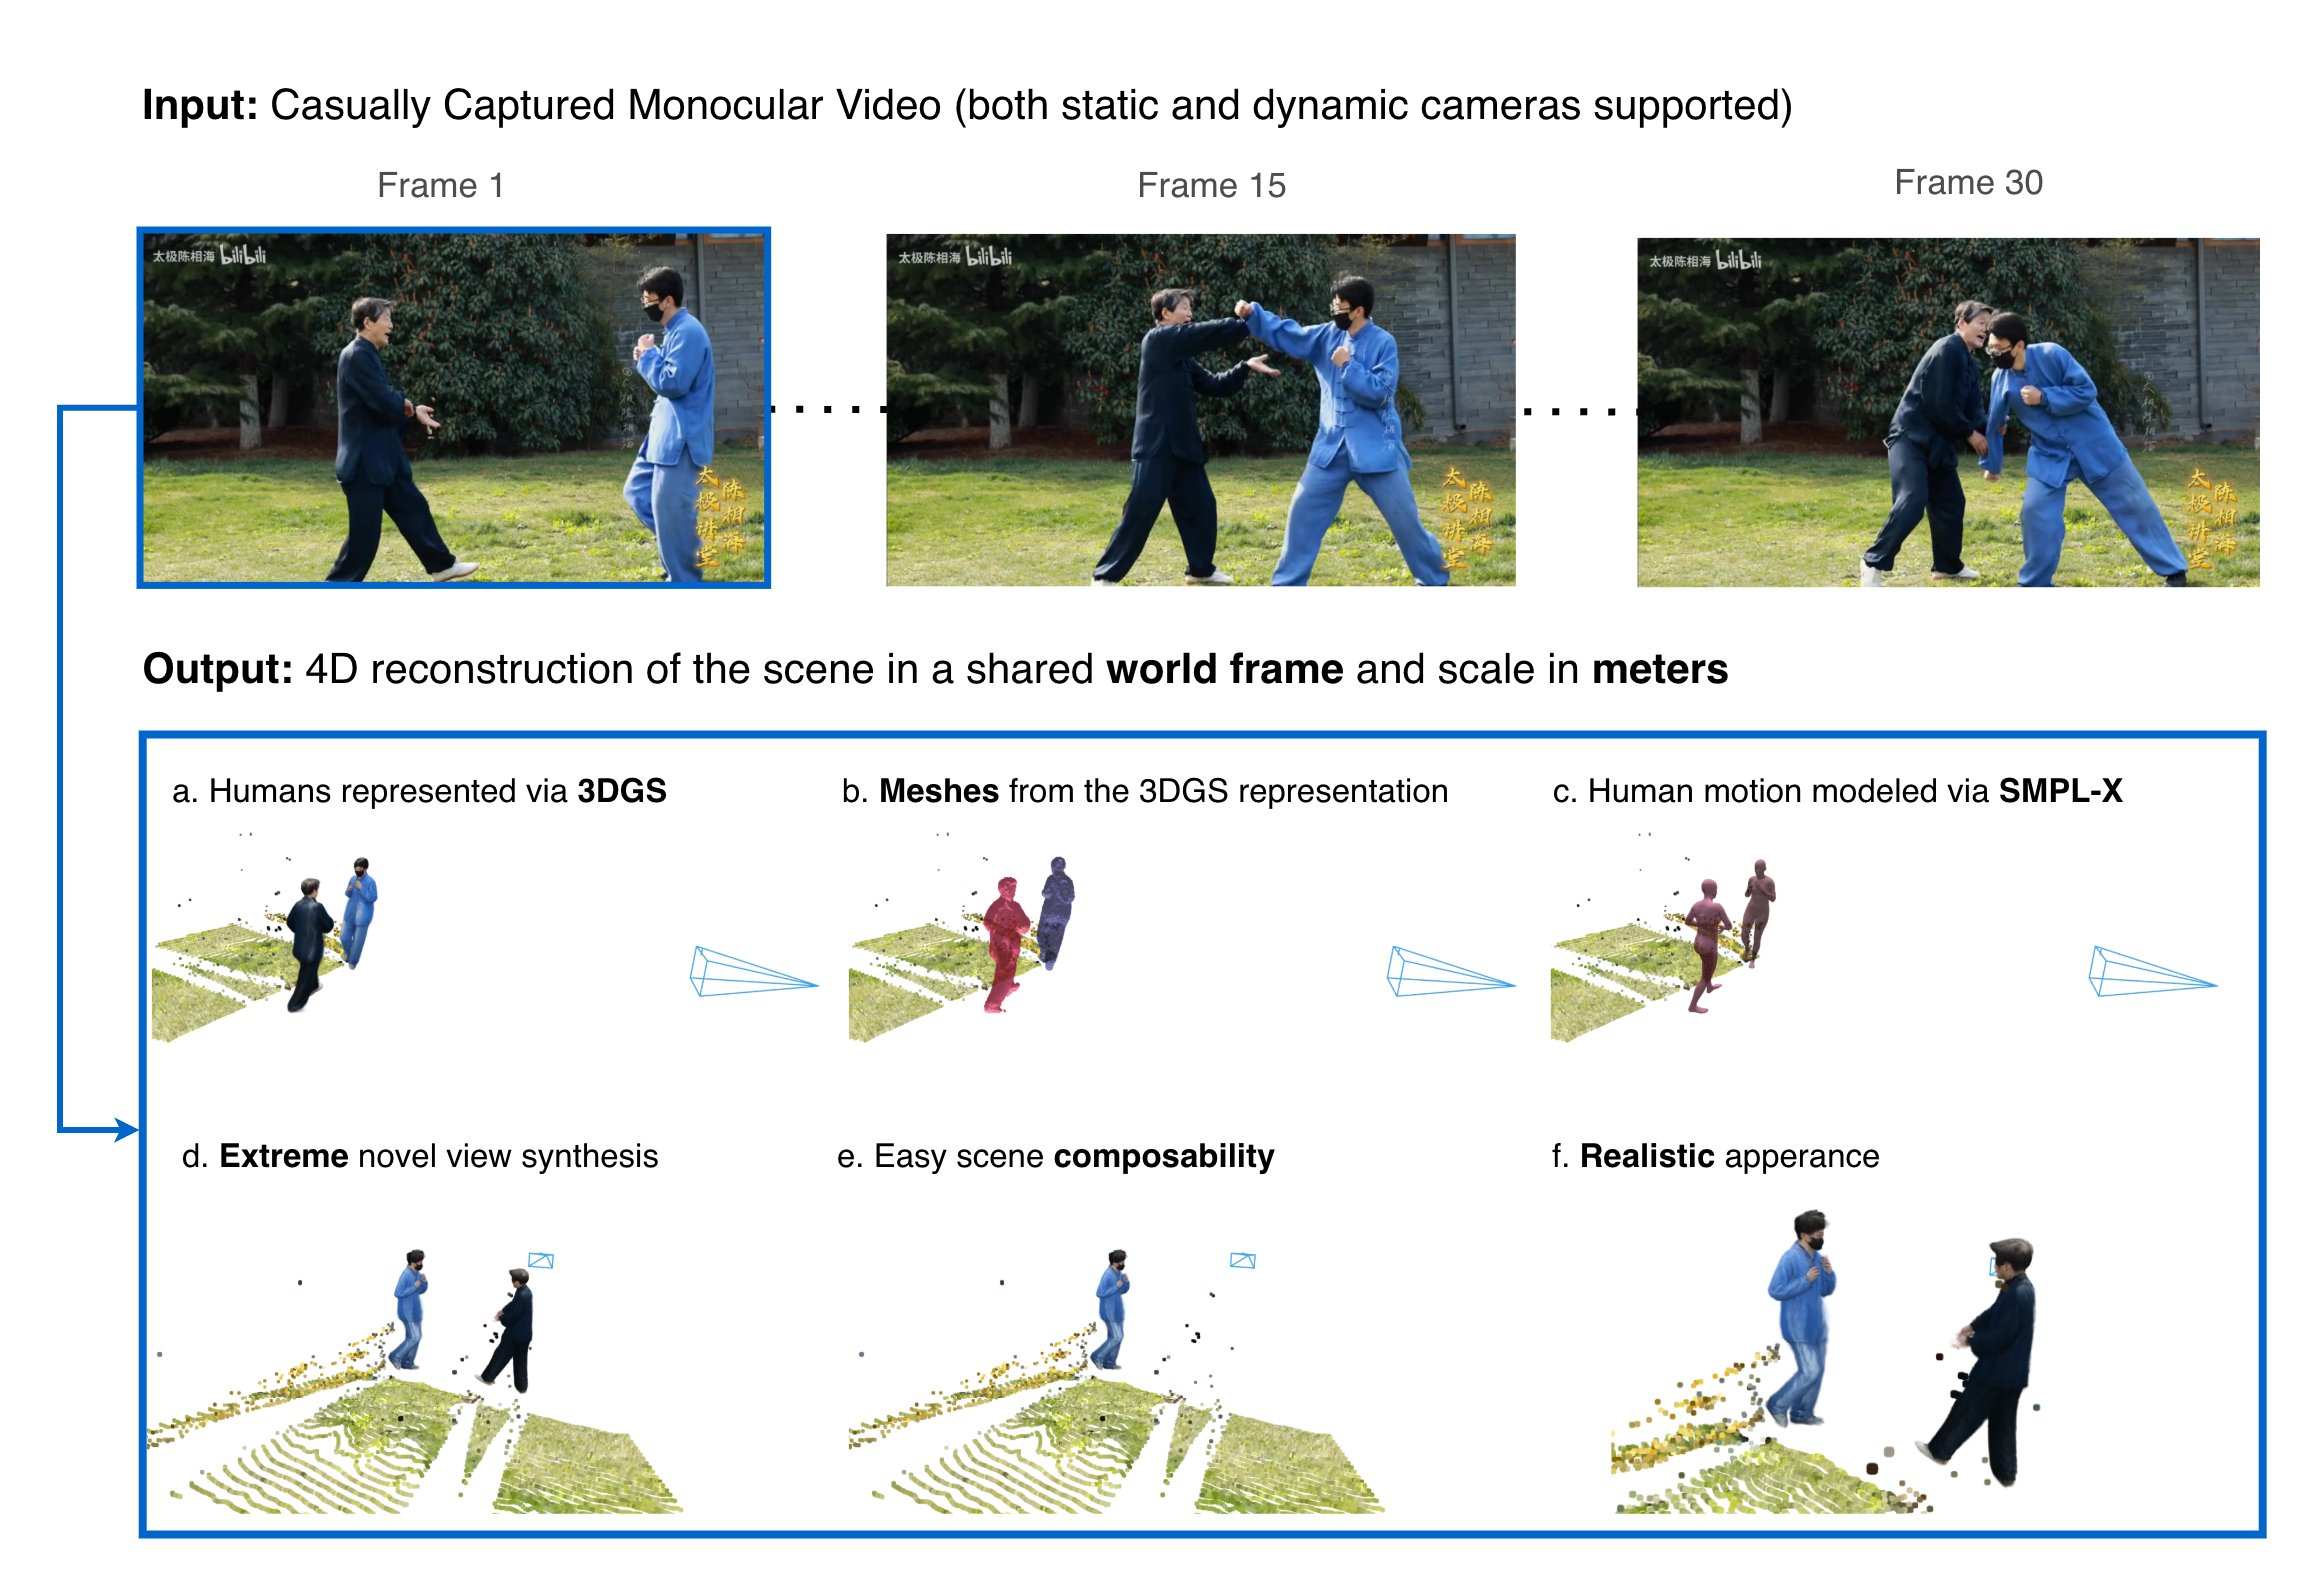
\includegraphics[width=1.0\textwidth]{figures/what_our_method_does_impress_fig.drawio.png}
    \caption{\textbf{High level overview of our method}. We propose a novel hybrid framework for monocular 4D reconstruction of dynamic human-centric scenes that combines the speed and efficiency of feed-forward networks with the accuracy and quality of optimization-based approaches. Given a monocular video of a dynamic human-centric scene, our method is able to reconstruct high-quality 4D scene representation that enables photorealistic novel view synthesis as well as accurate human motion extraction.}
    \label{fig:input_output_overview}  
\end{figure}

% Problem scope, and what my work is doing, and how it can be useful in real world applications
% We want to focus on *dynamic* human centric scenes captured from monocular video that capture multiple humans interacting or performing complex motions. 
% Our method is able to handle inputs from static as well as moving cameras, which is important for real world applications where the camera might be handheld. 
% I see two important applications of my work
% - First: interactive media - we no longer have to rely on watching monocular feed, and instead can view the given video from any angle we want. This is especially useful in sports broadcasting, where the viewer can choose their own perspective. Here, the important aspect of the reconstruction is how accurate the extracted motion is, and how realistic the novel view renderings are.
% - Second: With the recent advances in humanoid robotics, being able to precisely recover human motion from monocular videos can help extract training motion data for robots to imitate. Here, we only care about the accuracy of the recovered motion, and not so much about the visual quality of the renderings.

Specifically, in this work, we focus on reconstructing human-centric scenes captured by a monocular static or dynamic camera, and where multiple people might be interacting or performing complex motions. As Figure \ref{fig:input_output_overview} illustrates, our method outputs a world aligned 4D representation of the scene with scale in meters. Specifically, we represent each human as a set of 3D Gaussians which are deformed over time using the SMPL-X \cite{smplx} human body model. Apart from the 3D representation, our method also recovers camera poses and static scene background represented as point cloud. In addition, the 3D Gaussian representation is aligned with the underlying SMPL-X model, which allows us to extract accurate human motion in the scene which can enable markeless motion capture applications and motion retargeting in the context of humanoid robotics (e.g. VideoMimic \cite{videomimic}). Finally, our 4D representation also enables free view rendering of the scene which can unlock novel ways of consuming video content or producing music videos (e.g. A\$AP Rocky Helicopte music video).

% General challenges in dynamic scene reconstruction
% - In general, 4D reconstruction from monocular video is highly ill-posed problem
% - In addition, the system needs to be able to accurately disentangle the motion of camera and objects in the scene
% - Apart from obtaining multi-view consistency from monocular video
% - Further, we need to make sure we correctly separate dynamic and static parts of the scene - e.g. avoid having static background bleed into dynamic objects
% Specific challenges in human-centric reconstruction
% - Humans are highly non-rigid objects, with complex articulations and deformations including clothing dynamics and hair motion
% - when we have multiple people in the scene, we have to deal with inter-person occlusions and interactions  

In general, reconstructing dynamic scene from a monocular video is a highly ill-posed problem and as requires to get a lot of small subtasks right. First, we need to accurately disentangle the motion of the camera from the motion of the objects in the scene. Second, to obtain high quality novel view renderings, we need to ensure multi-view consistency along with predicting the unseen part of the scene. Futher, to obtain clean reconstruction of the dynamic and static scene, we need to correctly separate dynamic and static parts of the scene - e.g. avoid having static background bleed into dynamic objects. importantly, for the human centric scenes, it is importantly to also ensure valid human body shape and pose, which becomes especially challenging when humans interact and occlude each other. Finally, humans are highly non-rigid objects, with complex articulations and deformations including clothing dynamics and hair motion, which makes the reconstruction even more challenging. Our method addresses these challenges by combining state-of-the-art pretrained models along with a novel optimization based framework that refines these predictions to arrive at a high quality 4D reconstruction of the scene.

% Gap in existing methods
% - Majority of the existing human-centric scenes methods focues on mapping either single image, set of image or monocular video to parametric human model (SMPL, SMPL-X, etc.). These approaches assume clean video capture conditions and fail for the in the wild scenarios where we might have multiple people interacting and occluding each other. 
% - In the last year or two, there has been a new wave of papers that deviate from the tradional 3D reconstruction methods, and instead, train a feedforward network to directly map the input image or video to the target set of modalities, usually depth maps and camera parameters. The main limitation of these approaches is that while at a first glance they give decent predictions, they are still much less acurrate than their more classical optimisation based counterparts. 
% - In addition, the feed forward methods often only estimate point clouds or meshes, which are not ideal for photorealistic novel view synthesis due to their discrete nature. Similarly, it is impractical to extract accurate joint positions from these representations, which is crucial for many applications such as motion capture for robotics.
% - While there have been previous attempts for monocular 4D reconstruction of dynamic human centric scenes, the main limitation of these approaches is that they require order of hours to days of training time per scene, making them impractical for real world applications. 


Existing human-centric methods focus on obtaining high quality avatar from a cleanly captured single image or a set of images \cite{anigs,gas,qiu2025lhm}, or monocular video \cite{humannerf,neuman,guo2023vid2avatar,exavatar}. In contrast to these methods, our work assumes multiple people in the scene which may interact, occlude each other and perform complex motions, making our setting much more difficult due to these factors. Further, while there have been previous attemts to deal with a similar setting to ours, most notable MultiPly \cite{multiply} and Guess The Unseen \cite{gtu}, these methods are order of magnitudes slower than our approach, requiring hours to days of training time per scene, making them impractical for real world applications. 

In contrast to the human-centric methods that make use of the parametric human body models such as SMPL \cite{smpl} or SMPL-X \cite{smplx}, there also exist generalist methods such as Shape-of-Motion \cite{som} which similar to our method make use of pretrained tracking model to define the deformation field of the dynamic objects in the scene. However, while the generalist methods are appealing, the pose and shape quality of the reconstructed humans is worse than the methods that rely on parametric human body models such as ours. Lastly, we also have feedforward methods which apart from being generalist, also drop the per scene optimisation and directly map the monocular video to the desired 4D representation. However, similar to the generalist methods, these feedforward methods also lag behind in terms of reconstruction quality compared to optimization based methods. In contrast to these methods, we build our method with concrete applicatiosn in mind, and therefore choose to build human centric method with high quality reconstruction as the main goal, while still being able to reconstruct a scene in order of minutes rather than hours to days. 


% Contributions
% - The main contribution of this work is a novel hybrid framework for monocular 4D reconstruction of dynamic human centric scenes that combines the best of both worlds - the speed and efficiency of feedforward networks, and the accuracy and quality of optimisation based approaches.
% - As a result, we obtain the quality comparable to the state of the art methods that require hours to days of training time, while being able to reconstruct a scene in order of minutes.
% - Our methods can not only obtain high quality novel view renderings, but also accurately recover human motion in the scene, making it suitable for a wide range of applications including interactive media and robotics
% - We directly address to limitations mentioned in MultiPly: to introduice generative prior and also to use more expressive human model SMPLX
% - We demonstrate our effectivness on our method on 4 tasks including human pose estimation, novel view synthesis, mesh reconstruction and segmentation 


In summary, the main contributions of this work are:
\begin{itemize}
    \item We propose a novel hybrid framework for monocular 4D reconstruction of dynamic human centric scenes that combines the speed and efficiency of feed-forward networks with the accuracy and quality of optimization-based approaches.
    \item Our method is able to reconstruct high-quality 4D scene representation that enables photorealistic novel view synthesis as well as accurate human motion extraction, making it suitable for a wide range of applications including interactive media and robotics.
    \item We directly address the limitations mentioned in MultiPly \cite{multiply} by introducing generative priors and utilizing the more expressive SMPL-X \cite{smplx} human model.
    \item We demonstrate the effectiveness of our method on four tasks including human pose estimation, novel view synthesis, mesh reconstruction, and segmentation
\end{itemize}
